\capitulo{5}{Resultados}

Una vez completado el proceso de desarrollo del proyecto, se debe realizar un análisis de los resultados obtenidos. De esta forma, se comprueba la eficacia y eficiencia del trabajo realizado en relación a los objetivos planteados al inicio.

\section{Resumen de resultados.}

El trabajo realizado ha logrado con éxito la creación de una herramienta que avanza en la monitorización de la EP. El desarrollo central ha sido una página web que facilita el control inalámbrico del dispositivo de recopilación de datos, e implementa nuevas funcionalidades para sus usuarios.

Esta plataforma web gestiona de forma eficaz la información de los diferentes tipos de usuarios registrados. Su interfaz implementa dicha gestión, ofreciendo funciones de creación, eliminación, modificación y consulta de información personal, así como de los datos obtenidos de la monitorización. Cumpliendo con el objetivo principal del proyecto, se ha logrado la comunicación en tiempo real para la visualización de parámetros de la actividad en curso, pero es necesario seguir trabajando en la precisión del registro y procesamiento de datos del sensor para evaluar y mejorar la velocidad de comunicación. Además, se han generado estadísticas básicas sobre los datos de monitorización almacenados para cada paciente. La futura explotación de los datos almacenados aumentará la utilidad del sistema, convirtiéndolo en un herramienta de valiosa para la toma de decisiones médicas objetivas en el tratamiento de pacientes con EP.

Para la implementación de estas funcionalidades, ha sido imprescindible lograr una conexión fiable a través de Bluetooth, diseñar y desarrollar una base de datos adaptada a las necesidades del sistema, y crear una interfaz comprensible y accesible para todos los usuarios.

A pesar de que no era un objetivo principal, se ha logrado una mejora significativa en el prototipo hardware. El dispositivo obtenido facilita la movilidad en la realización de pruebas y presenta una autonomía completa, asegurando la seguridad y manejabilidad del prototipo. El montaje final se muestra en la Figura \ref{fig:hardwareFinal}.
\begin{figure}[h]
    \centering
    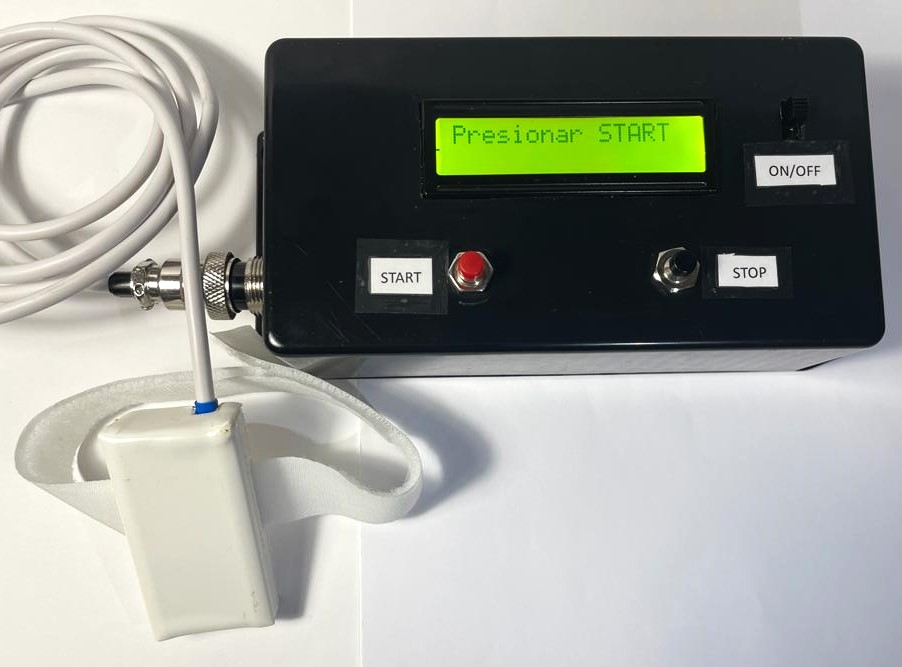
\includegraphics[width=0.7\textwidth]{img/E1_Planos/montajeFinal.jpg}
    \caption{Hardware del dispositivo final.}
    \label{fig:hardwareFinal}
\end{figure}


\section{Discusión.}

Los resultados de este proyecto son una fuente de innovación y mejora respecto a otros trabajos del ámbito de la monitorización de la EP. Uno de los mayores avances es la creación de una interfaz web multifuncional, que admite distintos tipos de usuarios (administrador, profesional y paciente) permitiéndoles gestionar su información. La plataforma también proporciona estadísticas personalizadas y comprensibles, con un diseño que asegura la accesibilidad de usuarios con diferentes competencias tecnológicas. Otra característica diferenciativa es su enfoque en el uso de los datos de monitorización de la marcha para la práctica clínica como apoyo en la toma de decisiones informadas. Estos datos también son de utilidad para los pacientes, y el proyecto contempla la integración de un sistema de alarma que les ayude a manejar situaciones de bloqueo en la marcha.

Para evaluar la usabilidad\footnote{facilidad con la que un sistema puede ser usado para llevar a cabo las tareas que se le requieren} de la aplicación web desarrollada, se considera oportuno diseñar y completar una SUS (System Usability Scale\footnote{Escala de Usabilidad del Sistema}). La SUS es una herramienta simple y confiable que, a través de un cuestionario de diez elementos, permite una evaluación rápida y de bajo coste. Utilizando este cuestionario se abordan diferentes aspectos de la usabilidad de la web, lo cual aumenta la validez y fiabilidad de los resultados y conclusiones derivadas de su uso \cite{SUS}. La puntuación SUS obtenida tras la evaluación fue de 97.5 sobre 100, superando sin lugar a dudas el punto de referencia estándar (68), y confirmando la obtención de una plataforma web que cumple con creces sus objetivos. La encuesta y sus resultados pueden consultarse en el Anexo \textit{G.1-Detalle de los resultados}.


    
